\chapter{Selective Registration}
\label{cha:Lush_Chapter_16}
\index{Culling levels|(}
\index{Selective registration|(}

In nearly all breeds of livestock in the United States every animal
which has a registered sire and a registered dam is eligible to registry
unless it has one of the few disqualifications which exist in some breeds.
Of course, many eligible animals do not get registered; but the decision
to register or not to register is left entirely to the breeder. It is occasionally
proposed that each animal ought to be inspected and approved by
authorized judges or ought to comply with certain minimum standards
of production, where those are appropriate, before it is finally accepted
for registration. This is selective registration.

This would be a special application of mass selection. No new principles
of inheritance are involved. The diagrams in Figure~\ref{fig:Lush_Figure_28}
show how various proportions of the population might be affected by such a plan.
Diagram \textit{A} shows the impossibly extreme case where the official inspection
could be perfectly accurate in eliminating the animals with the
lowest breeding values. Diagram \textit{B} shows, with areas of the same size,
how the real breeding values might very well be distributed in the case
where individual merit is only moderately correlated with breeding
value. Some of those which would be eliminated by selective registration
would be superior to some of those which would be accepted. That
is inevitable wherever outward individual merit is not perfectly correlated
with breeding value. The proportions of the different areas in
these diagrams are not particularly important. Those vary from breed
to breed and from time to time and are different for males and
females.\footnote{In the cattle breeds the number of males registered in
recent years has generally been about one-half to one-third as large as
the number of females registered.}

\begin{figure}
	\centering
    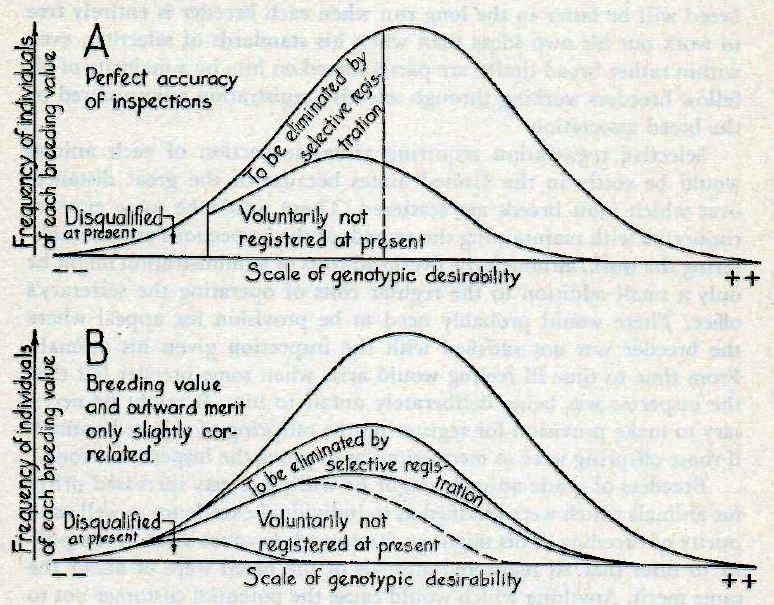
\includegraphics[width=\textwidth]{Figure_28.png}
    \caption{How the distribution of a population might be affected by selective
			 registration. Corresponding areas are the same size in the two diagrams.
			 The areas in each diagram are exclusive of each other. \textit{A}
			 presents the impossibly extreme case where the inspections could be
			 perfectly accurate. \textit{B} presents a more probable situation
			 where many mistakes would be made by the inspectors although they would be
			 right oftener than they would be wrong. If many were eliminated by the inspectors,
			 it might be necessary to register some of those voluntarily not registered at present.
			 Those would come from the areas just to the right of the dotted lines.}
    \label{fig:Lush_Figure_28}
\end{figure}
\index{Culling levels|)}

Both diagrams indicate that the animals not now registered include
many which are of higher breeding value than some of those which are
registered. It is probable that the average breeding worth of those registered
is higher than the average breeding worth of the eligible ones
which do not get registered, although the difference may not be as
extreme as is pictured here. Selective registration would increase the
intensity of selection for those genes which would usually make their
possessors appear more desirable to the inspectors. This would increase
slightly the rate of improvement in the breed, as far as mass selection
can do that and as far as the ideals set up to guide the inspectors are in
agreement with real merit. Whether the amount thus gained would be
sufficient to make selective registration worth the money and effort it
would cost is open to some doubt.

Selective registration would have some tendency to unify the standards
of selection within each breed, since each breeder would have to
be guided in part by the ideals of the inspectors. Those might not
always be superior to his own. This control over standards of selection
might do actual harm by preventing individual breeders from trying
out their own ideas as freely as they would like. To understand that,
one has only to imagine what would have happened if there had been
an official system of inspection in the Shorthorn breed when the Cruickshanks
were founding the``Scotch'' type or in the Poland-China breed
when Peter Mouw was forming the ``big type.'' The help which the
inspectors would give many breeders in their selections might more
than offset this. Moreover, the inspectors would probably be lenient
enough to allow each breeder considerable leeway for his own standards.
It remains an open question whether the average progress of the
breed will be faster in the long run when each breeder is entirely free
to work out his own ideas than when his standards of selection, even
within rather broad limits, are partly forced on him by a majority of his
fellow breeders working through selective registration administered by
the breed association.

Selective registration requiring visual inspection of each animal
would be costly in the United States because of the great distances
over which most breeds are scattered. There would be some expense
connected with maintaining the records of the inspections and administering
the work, although the overhead costs of administration might be
only a small addition to the regular costs of operating the secretary's
office. There would probably need to be provision for appeal where
the breeder was not satisfied with the inspection given his animals.
From time to time ill feeling would arise when some breeder felt that
the inspector was being deliberately unfair to him. It might be necessary
to make provision for registering the offspring of rejected animals
if those offspring were so meritorious as to prove the inspectors wrong.

Breeders of grade animals might be willing to pay increased prices
for animals which were certified as to individual excellence as well as to
purity of breeding. This might go far enough to cause some of the public
to infer that all registered animals of the breed were of about the
same merit. Anything which would cause the potential customer not to
study the animals before he makes his selection, or which would tend to
minimize attention to the breeder's reputation, has its possibilities of
doing harm. It seems unlikely that selective registration would be carried
far enough to make this danger important.

One commercial aspect of the situation is that some owners make
more strenuous efforts than others to sell males to other breeders of
purebreds. A certain amount of overhead in showing, advertising, and
sales efforts is required to sell any large fraction of the males produced.
In some cases those who make such efforts try hard to sell nearly all the
males they produce, while others make little effort to sell males except
to breeders of grades. The herds concerned usually do not differ that
much in real breeding merit. The adoption of selective registration
might restrict the efforts of those who are most active in selling males
more than it would those who are not now active at that. Doubtless
other unforeseen effects and complications will develop when selective
registration is put into practice. Any association attempting it will need
a trial period of several years to gain the experience necessary for making
the plan operate successfully when applied to the whole breed.

From 1942 to 1944, the American Jersey Cattle Club admitted bulls
to registry only if their paternal sisters or their dams had met certain
production requirements or if the sire was a ``star'' bull. The sire
becomes a star bull by his ancestors having met certain production
requirements or if at least ten of his paternal sisters and his dam have
been classified officially as to type and have scored high enough. There
are four grades of starring, the four-star bulls having the most promising
pedigrees, three-star bulls next, etc. In addition there are the
unstarred bulls which have not enough production or type ratings
among their near relatives to earn them even one star. Since 1944 the
compulsory features involved in selective registration. have been
dropped but the starring plan is retained. Since 1944 the Ayrshire association
lists progeny-tested sires in three classes of apparent merit but
what the breeder does with this listing is optional with him.

\section*{SELECTIVE REGISTRATION IN OTHER COUNTRIES}

Selective registration is practiced in many of the continental European
countries. The rules for operating the plan vary but in general are
somewhat as follows. The inspectors work under the direction of the
farmers' co-operative societies or of the breed association. In either case
there is usually some financial support from the government, accompanied
by a small amount of governmental supervision to see that such
money is spent in accordance with the laws appropriating it. The breed
association maintains tentative registry books and permanent registry
books. Soon after an animal is born it is entered in the tentative registry
and at an appropriate time an inspector certifies to this animal's individual
merit. It may then be placed in the permanent registry, or in
some cases it may remain in the tentative registry as long as it lives and
be placed in the permanent registry only after its death . Naturally the
animals are not inspected until they are grown or at least well along
toward maturity so that the inspector can be fairly certain of their
mature individuality. Tentative registry is therefore necessary to keep
the records straight. In the case of dairy cattle it is usually required that
females shall produce a minimum quantity of milk or fat before they
are finally placed in the permanent register and that males to be eligible
for the register must be out of cows which have met production
requirements higher than the minimum requirement which would
entitle cows to entry. Sometimes the inspection by the committee takes
place at the local fairs and sometimes the inspectors go from farm to
farm systematically or upon request.

The countries where these selective registration systems are in operation
are mostly countries where the breeds are native, and therefore the
ancestry of the majority of the commercial stock differs only slightly
from that of the pedigree stock. This makes more need for setting off,
by some special requirement or inspections, those animals good enough
to furnish future breeding stock than has been the case in the United
States, where most of the pure breeds have been imported and at first
differed greatly from the stock in the communities where they were
introduced. In most of the countries where selective registration is in
effect, the formal organization of the breed association occurred at a
comparatively recent date. This contributes something to the feeling
that there is no great gulf between the registered and the unregistered
animals. Usually provision is made for admitting to registry high grades
which are outstanding in their individual merit.
\nowidow

The following special items about selective registration in some
other countries may suggest the special conditions encountered and the
variety of ways adopted to meet them. They are by no means a complete
account of the registration systems in use. The details of those are
changed from time to time.\footnote{This is written in May, 1945.}

\textsc{Germany}. German animal breeding practices and customs of registration
were, of course, thrown into confusion by the war of 1914--18.
The cow-testing associations and similar organizations were again
operating on an extensive scale by 1924 or soon afterward. Since 1930
only cattle from herds which have been in cow-testing association work
have been eligible to be shown at the national exposition. Since 1934
and especially since 1936 the compulsory features of cow testing have
been greatly extended. In Hanover about 18 per cent of the cows were
tested voluntarily in 1934, but under compulsory testing this rose to 83
per cent by the beginning of 1937. The German animal breeding law
of 1936 brought about far-reaching control and compulsory inspection
(Korung) of all classes of breeding stock. In many cases only one or two
breeds could be kept in each district. This extended to sires used only
in private herds, as well as to sires which were offered for public service.
This system was not in operation long enough before the next war to
demonstrate what effects it actually would have.

\textsc{Holland}. The Netherlands Herdbook Association\footnote{The Friesian
Cattle Herdbook Association (with headquarters at Leeuwarden) has a slightly
different procedure.} at the Hague maintains four kinds of herdbooks: the
calfbook, where service certificates and \index{Birth certificates}birth certificates are filed in
order to keep the records of ancestry straight; the herdbook proper, to which
animals are admitted on mature inspection; the advanced register for recording
production; and the register of proved sires. The filing of service certificates
soon after breeding is compulsory. The filing of the birth certificate must take
place within a few weeks after the birth of the calf. Females are
inspected and scored for entry into the herdbook proper soon after they
drop their first calf. A score of 75 points out of a possible 100 is necessary
for registration. Recording milk and fat production is not compulsory,
but bulls are not accepted for registry unless they are from
tested dams. Bulls are inspected and scored soon after they are 12
months old, before they go into service, but must be scored again after
they are 24 months old. If a bull is accepted as a yearling but is rejected
at the two-year-old scoring, the owner is allowed 30 days as a reasonable
time in which to get another bull. All services made by the rejected bull
more than thirty days after his rejection are treated as though the bull
were a grade, but services made prior to that are accepted for purposes
of registration. The inspection is so severe that about 55 per cent of all
bulls offered for inspection are rejected. There is, of course, no way of
judging how much selection the breeders have already practiced in
deciding which bulls shall be offered for inspection.

\textsc{Switzerland}. In Switzerland the physical conditions, especially the
summer use of mountain pastures far from the home villages and the
small size of many of the herds, compel more co-operation among
breeders than is usual in the United States. Bulls must be shown at the
large regional fairs for classification if the purchasers are to be eligible
to receive the payments which the government provides for stimulating
the use of improved sires. Such payments and other considerations are
important enough that almost all bulls get shown at these large regionai
shows. Frequently as many as 1,300 Brown Swiss bulls are shown at one
time at the largest fair. The cows are offered for inspection at the local
or village fairs. Cows are scored during their first or second lactations,
and those scores are printed along with their pedigrees in the printed
herdbooks. The advanced registry records not only how much milk and
fat the cow gave, but also how many hours she worked at draft purposes
during the year. A considerable fraction of the Swiss cattle are used for
milk, work, and beef, thus being in a sense triple-purpose cattle. Special
stress is laid on longevity and regularity of breeding . Each cow which
produces at least six living calves in the space of eight consecutive years
is given a special distinguishing mark in the printed herdbook.

\textsc{Denmark}. In Denmark there is widespread co-operation among
farmers for many purposes, and the co-operative societies conduct the
pedigree registration and other means of livestock improvement. Breed
registry societies, such as those in the United States and Britain, do not
exist. A committee of the union of co-operative societies directs the registration
policies as the board of directors of a breed association would
do in the United States. Of course, most members of this committee are
breeders themselves or have in some other way made themselves thoroughly
familiar with the practical problems which breeders encounter.
Hence, the conduct of registration is not very different from that in the
United States; but the committee members are responsible to the farmer
co-operative societies, that is, to the customers who will use the
improved breeding stock being produced. It has been agreed that 500
cows registered per year is a large enough number to supply the real
needs of the breeders and farmers. The animal husbandry \textit{consulents}
\footnote{Employees of the co-operative societies who provide technical
advice on livestock matters, somewhat as county agricultural agents do in
the United States, and also act to some extent as the business agents for
their co-operatives.}
nominate something like twice that number of cows. Then the central
committees consider the available data concerning these and discard
those which seem least worthy until the number is reduced to 500. Cows
rejected one year can be nominated again and perhaps accepted in a
later year. No cow is considered until she has been in milk at least three
consecutive years. No matter what her age when nominated, her actual
uncorrected fat production must have averaged more than 400 pounds
per year ever since she first freshened. The national committee in
charge of swine breeding supervises the registration of swine. Registrations
are accepted only for animals bred at the state-recognized swine
breeding centers. Those are farms where the breeders have complied
with certain regulations, including sending each year to the testing stations
half as many test litters as they have sows in their herds.\footnote{Lush,
Jay L. 1936. Genetic aspects of the Danish system of progeny-testing swine.
Iowa Agr. Exp. Sta., Res. Bul. 204.} At the testing stations these test litters
(of four pigs each) are fed under standard conditions, and the rates and
economy of gain are recorded. When each pig reaches 200 pounds, it is
slaughtered at a nearby bacon factory and its dressing percentage and the type,
conformation, and quality of its carcass are measured and scored. Also, each
breeding center is inspected twice each year by a committee which scores it
for: (1) management and general appearance of the farm, (2) conformation of the
breeding animals, (3) fertility of the breeding animals, (4) efficiency in the
use of feed by the test pigs from this center, and (5) slaughter quality of the
test pigs from this center. The considerable costs of the swine improvement plans
are mainly borne by the co-operative bacon factories. The plans are thus directed
and financed indirectly by the customers who buy the improved breeding stock and
not by the breeders who produce it. The government makes a small financial
contribution to part of the work and extends legal authority where needed to the
co-operative societies or to the co-operative bacon factories but does
not itself take an active part in directing the work. Exhibiting at the
fairs is not compulsory, but a large part of the breeders do that. The
classification made at the fairs is entered in the herdbooks or other records
pertaining to those animals, so that most pedigrees have in them
considerable information about the type classification of the ancestors,
especially of the sires. The central committees specify in detail the kind
of records which each stockman, who aspires to be called a breeder,
must keep. The committees or their representatives inspect those private
herdbooks at certain intervals for accuracy and completeness. In
some cases the owner is not permitted to make the entries himself but
must keep the notes and papers concerning each event until the consulent
comes on one of his regular visits, verifies them as well as he can,
and makes the proper entries. This supervision and uniformity give the
private herdbooks a semiofficial standing and make it unnecessary for
the central committee to keep birth certificates or other records of that
kind on animals not yet admitted to the national herdbooks.

These details will show something about how widely the pattern of
selective registration may vary from country to country according to
circumstances. If selective registration is adopted in the United States,
still other devices will be needed to adapt it to the local needs and
conditions.

\section*{AMERICAN APPROACHES TO SELECTIVE REGISTRATION}
\index{Breed associations|(}

The Standardbred horse is an American breed which takes its mime
from the fact that in its early history animals must have been able to
trot a mile in 2 minutes and 30 seconds or pace a mile in 2 minutes and
25 seconds before they could be registered. The Brahman Cattle Breeders
Association (founded in 1924 and operating mostly in the coastal
regions of Texas and Louisiana) requires inspection of animals before
they are accepted for registry. The scores and other descriptive comments
concerning each animal are filed with its registration in the
secretary's office. No herdbook has yet been published. When the Jersey
breeders established their Register of Merit in 1903, many of the cows
were measured and scored as to type by some member of a group of
about 19 authorized judges. These scores were not used, however, to
determine eligibility for registry. They were intended to furnish evidence
about the relation between type and production. Perhaps also
some of the breeders then feared that unfortunate results would follow
if the Register of Merit were allowed to operate with no attention at all
to type.

\textsc{Disqualifications}. Many breeds have certain absolute disqualifications
which are a bar to registry, even though the breeding is of
undoubted purity. Thus, an Aberdeen-Angus which is red is not now
eligible to registry; although red cows were eligible until about 1915.
Red Aberdeen-Angus steers may still be registered to compete for prize
money at the fairs. Neither is a red and white Holstein-Friesian nor one
with black completely encircling the hoof-head eligible to registry. Most
of these absolute disqualifications concern deviations from the peculiar
type of that breed, which usually means details of conformation or
color not directly affecting their usefulness as producers of meat, milk,
eggs, wool, or power. No association will knowingly register an animal,
either male or female, which is known to be a nonbreeder, except in the
case of fat animals and geldings to be exhibited at shows. In none of the
cattle breeds can a heifer born twin with a bull be registered until proof
is furnished that she is fertile. This restriction is based upon the common
experience that most such heifers \index{``Free-martin''}(``free-martins'') will be barren.
Years ago some of the breeds had rules against registering offspring
from dams which had formerly produced crossbred young to the service
of grade sires or sires of other breeds. Only a few breeders actually professed
a belief that this would affect the breeding value of subsequent
purebred offspring (``telegony'')\index{Telegony}, but the rule was placed in the by-laws
of many associations on the long chance that there might be something
to it. In 1924 it was removed from the by-laws of the last large association
(a sheep one) which had had this rule. Breeders of dogs are reputed
to believe more in telegony than breeders of other livestock.

\textsc{Age Restrictions}. Many American breed associations levy an extra
charge on registrations not made until after the animal passes a certain
minimum age. In some breeds the animals cannot be registered at all
after they pass a certain age. One reason for this is to complete the registration
before the breeder loses or forgets some of the facts in the case.
The opportunity for fraud is also diminished by having the registration
made promptly. More animals are registered than if registration could
be postponed indefinitely without penalty. One unfortunate result is
that some animals are registered young which would not be registered
if the breeder could wait until he could see them as mature animals. A
plan which promises to combine the advantages without the disadvantages
of early registration is ``deferred registration'' such as that in effect
with the Guernsey, Jersey, and Ayrshire breeds. Under this plan the
breeder files a birth certificate soon after the calf is born. The fee for
this is small. This birth certificate entitles the breeder to defer final
registration until the animal is mature, without incurring any penalty
for lateness.

\textsc{Voluntary Plans}. The voluntary Herd Classification plans of the
dairy cattle registry associations in the United States embody some
selective registration in the fact that the registration certificates must be
surrendered on animals classified as poor and that bulls out of cows
classified as fair are not eligible to registry. The Herd Classification
plan also records the animals in several different classes of individual
merit, so that one who does not know the animals may learn what the
classification committee thought of their individuality. The type classification\index{Type classification}
is printed, after the name and number of each classified animal,
in the various printed herdbooks. This puts more meaning in
pedigrees in which these classified animals appear.

A feature of selective registration in the Herd Improvement Registry
of dairy cattle is that the breeder who surrenders the registration
certificates for his poorest producers is entitled to have those omitted
from the published average for the production of his herd. The extent
to which this is actually being done may be seen from the fact that, in
the first 13 volumes of the Holstein-Friesian Herd Improvement Registry,
14,733 certificates of registry were surrendered voluntarily. This
was 10.3 per cent of the total number of cows on test. Of course, some of
these surrendered certificates were for cows already dead or barren.
Even so, the figures indicate some selective registration against the
least productive animals even after the expense of registration has
been met.

The Ayrshire Association registers bull calves under six months old
for half price if the sire and dam, or the dam and paternal grandam, or
all four grandparents are in the Ayrshire Advanced Registry.

Such individual registration of poultry as exists is mostly connected
with records of performance in such a way that it is selective.

\textsc{Abandoned Plans}. In 1889--91 the Holstein-Friesian Association
paid bounties of \$5 each for the castration or vealing of bull calves
which were eligible to registry. This was a systematic attempt to induce
the breeders to discard their ordinary and inferior male calves. The
plan was discontinued because nearly as many bull calves were registered
while the plan was in effect as before, and it was a heavy drain on
the association treasury, more than \$20,000 being thus expended in the
three years it was in effect.

The Hereford association in 1895 and 1896 had a rule that 10 per
cent of all applications for registry of bulls from each herd should be
rejected, but the Secretary had no guide as to which ones those should
be. The ruling was repealed in 1897.

\section*{SUMMARY}

Selective registration is a form of official mass selection which consists
in preventing individuals deemed inferior from leaving any registered
descendants. Such selection cannot do any more than the individual
breeder could; it may do more than he would if left entirely to
his own initiative. Collective wisdom, as imparted by the inspector,
might help the less well informed and might be of considerable help to
the customer. Probably it could not rise to the level of the ablest individual
breeder's ability.

Selective registration is widely practiced in many foreign countries,
but some of their conditions are distinctly different from those in the
United States.

Some of the American associations are experimenting with devices
embodying some voluntary principles of selective registration. Doubtless
these will be carried farther if they are found satisfactory and if the
problem of expense can be solved.
\index{Breed associations|)}

\section*{REFERENCES}
\begin{hangparas}{0.5in}{1}%
American Jersey Cattle Club. 1941. Selective Registration.

Gardner, Malcolm H. 1932. Selective herd-hook registration. Holstein-Friesian
World. 29:411--12 and 428.

Van den Bosch , I. G. J . 1930. The scoring system in the Netherlands. Holstein-Friesian
World, 27:337 et seq.

---. 1930. The Holstein industry in America. Holstein-Friesian World, 27:283.

Wriedt, Christian. 1930. Heredity in livestock. (Especially pp. 151--67). New York:
The Macmillan Company.
\end{hangparas}
\index{Selective registration|)}